\documentclass{LabReport}
\title{计算方法数值实验2-实验报告}
\author{221900180 田永铭}
\date{\today}
\addbibresource{refs.bib}
\Chead{计算方法数值实验2-实验报告 221900180 田永铭}
\Cfoot{\thepage}
\usepackage{listings}
\usepackage{graphicx} 
\usepackage{tikzsymbols}
\usepackage{tikz}
\usepackage{hyperref}

\lstset{
	basicstyle=\ttfamily, % 设置等宽字体
	frame=shadowbox,
	language=C,
	showspaces=false % 不显示空格
	showstringspaces=false % 不显示字符串中的空格
	showtabs=false, % 不显示制表符
}

\begin{document}
	\maketitle
	
	\section{实验题目}
利用matlab实现4阶Adams预测-校正方法的PECE模式算法求常微分方程初值问题:
\[
\left\{
\begin{aligned}
	&y^\prime = \frac{4x^2-2xy}{1+x^2}, \quad 0\leq x\leq5 \\
	&y(0) = 2 
\end{aligned}
\right.
\]
在$x_i = ih,i = 1,2,\cdots,50(h = 0.1)$点上的$y(x_i)$的近似值$y_i$,保留6位小数.用经典的4阶Runge-Kutta方法提供初始出发值$y_1,y_2,y_3$.\\
输出:列表输出 $i,x_i,y_i,y(x_i),y(x_i)-y_i$,输出结果要清晰.

	\section{实验原理}
	\begin{itemize}
		\item \textbf{实验原理——4阶Runge-Kutta:}4阶Runge-Kutta方法是利用泰勒级数推导出的高精度的单步法,其中经典格式用的最多,可以用它求解常微分方程的初值问题。它的表达形式如下:
\[
\left\{
\begin{aligned}
	&y_{n+1}=y_n+\frac{h}{6}(K_1+2K_2+2K_3+K_4),\\
	&K_1 = f(x_n,y_n)\\
	&K_2 = f(x_n+\frac{h}{2},y_n+\frac{h}{2}K_1)\\
	&K_3 = f(x_n+\frac{h}{2},y_n+\frac{h}{2}K_2)\\
	&K_4 = f(x_n+h,y_n+hK_3)
\end{aligned}
\right.
\]
		\item \textbf{实验原理——Adams—PECE:}基于数值积分,可以构造出Adams线性多步法,通过泰勒公式来分析误差,Adams显式格式和隐式格式能匹配四阶成Adams预测-校正(PECE)系统,它可以利用上述4阶Runge-Kutta方法来提供初值,然后根据以下公式来进行求解常微分方程的初值问题:
\[
\left\{
\begin{aligned}
	&P:\bar{y}_{n+1} = y_n + \frac{h}{24}(55f_n - 59f_{n-1} + 37f_{n-2} - 9f_{n-3}) \\
	&E:\bar{f}_{n+1} = f(x_{n+1}, \bar{y}_{n+1}) \\
	&C:y_{n+1} = y_n + \frac{h}{24}(9\bar{f}_{n+1} + 19f_n - 5f_{n-1} + f_{n-2}) \\
	&E:f_{n+1} = f(x_{n+1}, y_{n+1})
\end{aligned}
\right.
\]
	\end{itemize}
	
	\section{核心代码以及说明}
	\subsection{定义常微分方程函数和真实数值解函数}
\begin{lstlisting}[language=python,frame=shadowbox]
f = @(x,y) ( (4*x.^2-2*x.*y)/(1+x.^2) );
exact_solution = @(x) (2+ (4/3)*x.^3)/(1+x.^2);
y = double(zeros(1,100));y(1) = 2;x = double(zeros(1,100));
h = 0.1;
for n = 1:51
	x(n) = 0.1*(n-1);
end
\end{lstlisting}	
	这部分定义了常微分方程函数和真实数值解函数,并在区间以步长为1取从0到50的点,注意matlab下表是从1开始的。
	\subsection{实现经典四阶Runge\_Kutta方法}
\begin{lstlisting}[language=python,frame=shadowbox]
% 利用经典四阶Runge_Kutta方法预测y2,y3,y4的函数
function [y2,y3,y4] = classical_Runge_Kutta(f,x,y,h)
	for n = 1:3
		K1 = f(x(n),y(n));
		K2 = f(x(n)+h/2,y(n)+h/2*K1);
		K3 = f(x(n)+h/2,y(n)+h/2*K2);
		K4 = f(x(n)+h,y(n)+h*K3);
		y(n+1) = y(n) + h/6*(K1 + 2*K2 + 2*K3 + K4);
	end
	y2 = y(2);y3 = y(3);y4 = y(4);
end
\end{lstlisting}
	由此我们可以求出初值$y_2,y_3,y_4$,而$y_1$是2已经有了。由这四个值我们就可以开始使用PECE系统了。
	\subsection{实现PECE系统}
\begin{lstlisting}[language=python,frame=shadowbox]
% 省去利用经典四阶Runge_Kutta方法预测y2,y3,y4的代码,上面已经展示
y_bar = double(zeros(1,100));
f_bar = double(zeros(1,100));
for n = 4:50
    %预测
    y_bar(n+1) = y(n) + h/24*(55*frac(n)-59*frac(n-1) ...
         +37*frac(n-2)-9*frac(n-3));
    f_bar(n+1) = f(x(n+1),y_bar(n+1));
    %校正
    y(n+1) = y(n) + h/24*(9*f_bar(n+1)+19*frac(n) ...
         -5*frac(n-1)+frac(n-2));
    frac(n+1) = f(x(n+1),y(n+1));
end
\end{lstlisting}
	简单代入公式即可实现。
	
	\subsection{优化PECE系统的实现}
	注意到,上面PECE系统的实现开了很多的变量空间,这样十分浪费空间。而老师上课所讲的是可以只用4个存储空间来实现类似的代码,具体做法是:只记录$y_1,y_2,y_3,y_4$四个值,在一步更新后用后一个值写入前一个,将结果写入最后的$y_4$。同时,$y\_bar$和$f\_bar$变量其实也只需要一个空间,我之前完全浪费了空间。优化后的实现如下:
	\begin{lstlisting}[language=python,frame=shadowbox]
% 好的实现,frac这个存储预测值的地方只需要4个空间
frac = double(zeros(1,4));
% 好的PECE实现,省空间
for n = 4:50
	% 预测
	y_bar = y(n) + h/24*(55*frac(4)-59*frac(3) ...
		+37*frac(2)-9*frac(1));
	f_bar = f(x(n+1),y_bar);
	%校正
	y(n+1) = y(n) + h/24*(9*f_bar+19*frac(4) ...
		-5*frac(3)+frac(2));
	frac(1) = frac(2);frac(2) = frac(3);frac(3) = frac(4);
	frac(4) = f(x(n+1),y(n+1));
end
	\end{lstlisting}
	
	
	\subsection{处理结果输出}
	我既格式化输出了题目要求的各种结果,又画了一张图来展示预测值和真实值的相似度。具体代码如下:
	\begin{lstlisting}[language=C,frame=shadowbox]
% 格式化输出结果,结果通过命令行窗口查看,空格符号显示了出来
fprintf(' i   xi    yi      y(xi)      y(xi) - yi\n');
fprintf('---------------------------------------------\n');
for i = 1:n+1
	yi = y(i);
	xi = x(i);
	exact_yi = exact_solution(xi);
	fprintf('%2d  %2.1f  %7.6f  %7.6f  %.10e\n'
		, i-1, xi, yi, exact_yi, exact_yi - yi);
end
% 绘制图象,准确值为红色虚线,预测值为蓝色圆点
xx = linspace(0, 5, 100);  % 在 0 到 5 范围内生成 100 个点
yy = double(zeros(1,100));
for i = 1 : 100
	yy(i) = exact_solution(xx(i));
end
plot(xx, yy,'r--');
title('Plot of result');
xlabel('x');
ylabel('y');
grid on;
hold on;
plot(x, y, 'bo');  
hold off;
	\end{lstlisting}
	
\section{实验结果}
首先是数据结果的展示,图片如下:

\begin{figure}[h!] % 设置浮动环境
	\begin{minipage}[t]{0.48\textwidth} % 左侧 minipage,宽度为页面宽度的 0.48
		\centering
		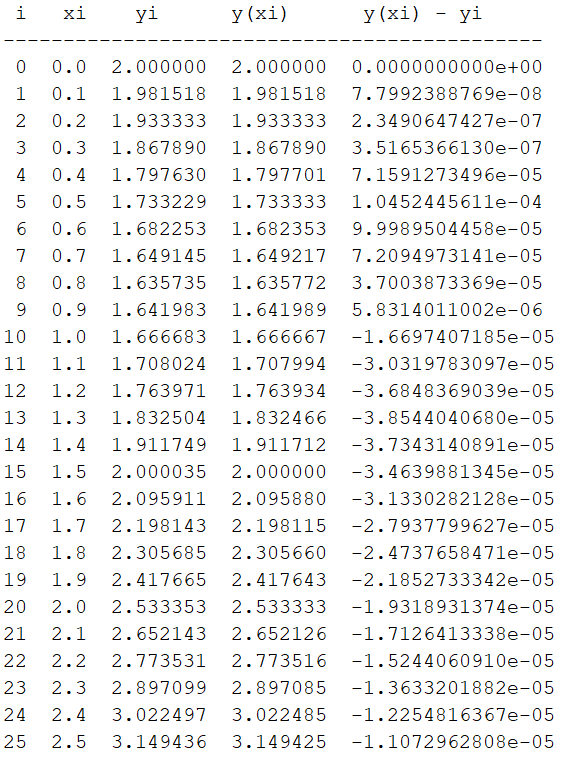
\includegraphics[width=\linewidth]{figures/result_table1} % 插入左侧图片
		\label{fig:left_image} % 左侧图片标签
	\end{minipage}
	\hfill % 水平间距
	\begin{minipage}[t]{0.48\textwidth} % 右侧 minipage,宽度为页面宽度的 0.48
		\centering
		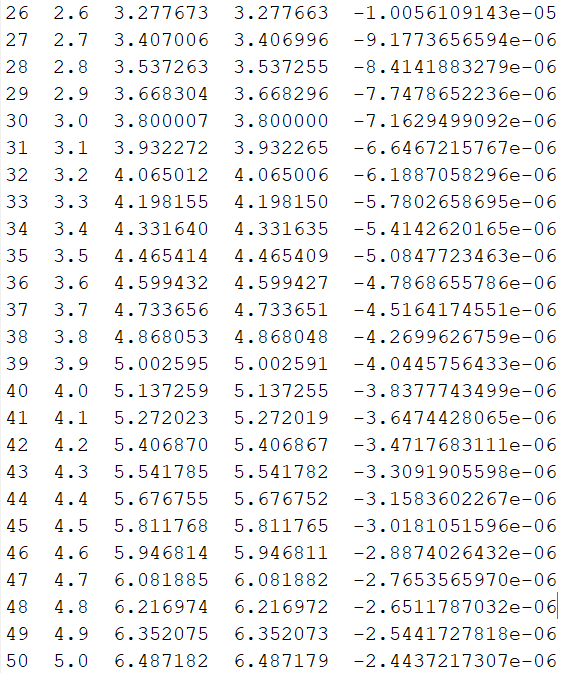
\includegraphics[width=\linewidth]{figures/result_table2} % 插入右侧图片
		\label{fig:right_image} % 右侧图片标签
	\end{minipage}
\end{figure}

\hspace{0em}然后是图象的展示,我的代码生成的图表中红色虚线为真实值,蓝色圆点为预测值。图象如下:
\begin{figure}[h!]
	\centering
	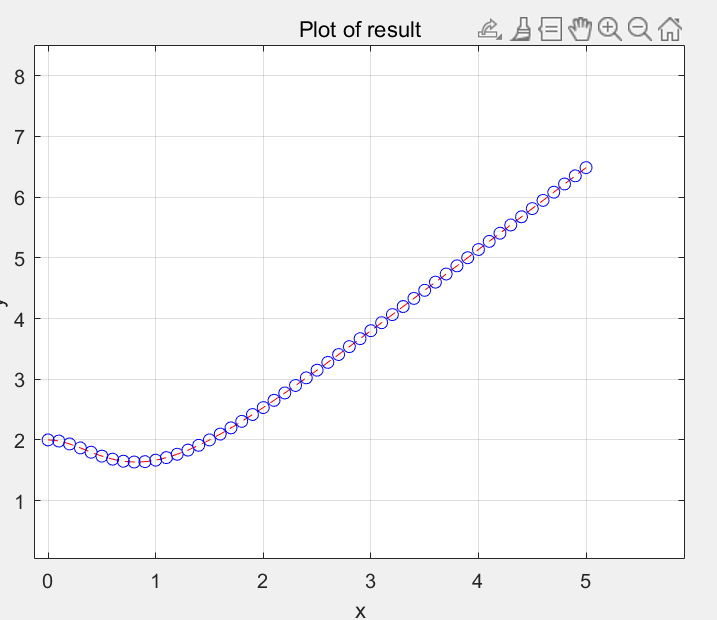
\includegraphics[width=0.5\linewidth]{figures/result_img}
	\label{fig:resultimg}
\end{figure}

	分析数据结果,可以知道,在保留6位小数的前提下,准确值和估计值的误差大概在1e-6左右,这已经是非常好的结果,这进一步说明了PECE方法的有效性。同时,我还发现,在计算该实验的常微分方程的表现上,PECE表现很好,随着点从0向5靠近,最后的精度甚至在提升,而一般的情况应该是精度越往后越差。当然这不是必然,因为我还验证了其他的函数,PECE也会出现越往后精度越差的情况。不过这个实验足以说明PECE方法的有效性。\par
	
	分析图表结果,可以观察到蓝色圆点几乎就正好落在红色虚线上,这说明PECE方法的预测值和真实值非常逼近。这也进一步验证了Adam-PECE方法的有效性。

\section{总结}

\begin{enumerate}
	\item 此次实验我全部采用matlab实现,全程独立实现无参考。我主动选择了使用matlab这个之前没怎么使用过的工具,了解了它的基础使用方法,并利用它完成了数值实验。正如老师所说,这是一款数学上的很好的工具,我为掌握它的基础用法而开心。
	\item 通过这次实验,我对Adams-PECE方法的理解更深了一步,理解了算法的原理、预测精确度、注意点和操作细节等等。
	\item 通过这次实验,我理论联系实际,将书本知识应用到程序上,激发了对计算方法这门课程的极大的兴趣。同时也明白了,数值实验是有误差的,是``差不多"的,但是做实验必须是仔细和精确到每一个细节的,例如我在优化Adams-PECE的时候,就是受到老师课堂的启发,主动降低了实验所需存储空间的开销,使得算法更加完美。
	\item 我还将实验结果进一步延展,利用我实现的方法来做书上一直在做的一个问题:
	\[
	\left\{
	\begin{aligned}
		&y^\prime = y - \frac{2x}{y}, \quad 0 < x < 1 \\
		&y(0) = 1 
	\end{aligned}
	\right.
	\]
	惊喜的是,得出了与书上PECE计算表格几乎完全一致的结果,这个结果也显然优于简单的Euler方法等方法。这进一步验证了这次实验的成功。
\end{enumerate}

\end{document}
